\documentclass{article}
\usepackage[utf8x]{inputenc}
%\usepackage{a4wide}
\usepackage[magyar]{babel}
\usepackage{times}
\usepackage{graphicx}
\usepackage[top=0.5in, bottom=0.5in]{geometry}
%opening
\author{Milán Unicsovics}
\title{MSc Önálló laboratórium 2}
\date{\today}
\sloppy
\begin{document}
%%%%%%%%%%%%%%%%%%%Szöveg%%%%%%%%%%%%%%%%%%%%%%
\thispagestyle{empty}
\begin{figure}[htp]
\centering
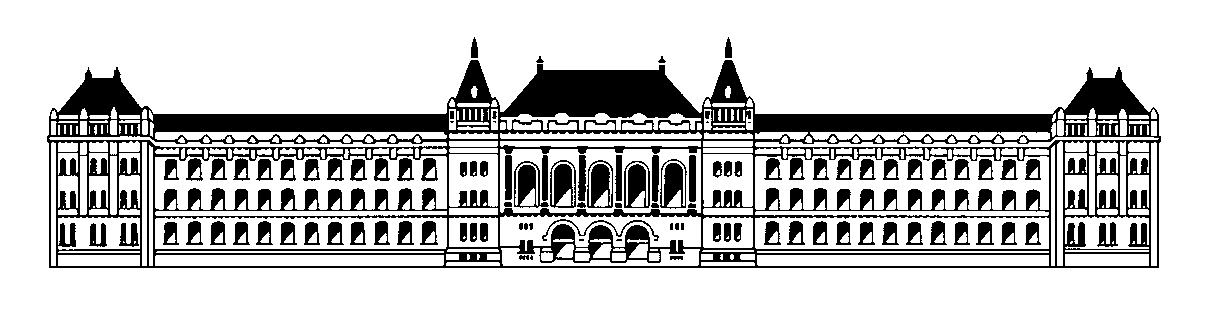
\includegraphics[scale=0.3]{img/bme.png}
\begin{center}
Budapesti Műszaki és Gazdaságtudományi Egyetem\\
Méréstechnika és Információs Rendszerek Tanszék
\end{center}
\end{figure}
\vspace*{-0.1in}
\begin{center}
\subsection*{Tesztgenerálás állapotgép alapú modellekből}
{\bf
Unicsovics Milán György (M9GNTV, I. évf, MSc) mérnök inf. szakos hallgató\\[0.3cm]

Konzulens: Dr. Micskei Zoltán adjunktus, MIT\\[0.3cm]

Szolgáltatásbiztos rendszertervezés szakirány 

Önálló laboratórium 2 összefoglaló 

2014/15. I. félév
}
\end{center}
\vspace{0.5cm}

A tesztelés célja a hibadetektálás, mely során egy szoftver elvárt és aktuális működését összehasonlítjuk. A modell alapú tesztelés ennek egy változata, ahol modellekel írjuk le a tesztelni kívánt szoftver viselkedését. A modellekből tesztek generálhatóak, melyek később futtathatóak a szoftveren. Kutatásaim célja, hogy későbbiekben egy olyan eszköz fejlesztésébe kezdhessek, mely állapotgép alapú modellt használó szoftverekhez tesztelő keretrendszerként használható.

Az előző félév feladata a modell alapú tesztelés elméleti hátterének és a modell alapú tesztelési folyamat megismerése volt. Ezen ismereteket az elérhető ipari tesztelő eszközökkel való ismerkedéssel folytattam. A megszerzett tapasztalatokat végül egy példa szoftver implementációjában foglaltam össze, mely egy kis projekten szemlélteti a modell alapú tesztelést.

Az idei félévben először egy hosszú távú célt határoztam meg és konkrétizáltam a tervezett tesztelő keretrendszer elkészítésének lépéseit. A készítendő keretrendszer egy Eclipse pluginként lesz elérhető, melyben Eclipse Papyrus állapotdiagrammokkal modellezett szoftverekhez lehet teszteseteket generálni.

Az elkészített állapotdiagramm modelljén azonban nem lehet azokat az alacsony szintű teszteset generáló algoritmusokat futtatni, melyek az absztrakt teszteseteket előállítják. Ezért szükség van egy köztes modellre, melyeken ezek az algoritmusok működhetnek. A félév fő feladata számomra tehát, köztes modellek és tesztgenerálási algoritmusok vizsgálata volt, melyeket főleg irodalomkutatás és az elérhető eszközök tanulmányozásával értem el.

Elsőként átfogóan vizsgáltam a tesztgenerálási algoritmusokat, melyek különböző megközelítéseket alkalmaznak: szimbolikus végrehajtás, modell alapú tesztgenerálás, kombinatorikus tesztelés, véletlenszerű tesztelés, keresés alapú tesztelés. Ezen technikák valószínűleg valamilyen kombinációját érdemes a siker érdekében használni.

A köztes modellek alkalmazását az ipari eszközökön keresztül kezdtem megismerni. A korábban vizsgált két eszközt is újabb nézőpontból vizsgáltam meg, koncentrálva a felhasznált modellre és felhasznált tesztgenerálási algoritmusra. Ezeket a tapasztalatokat egészítettem ki három új eszköz elemzésével. Az általam különösen behatóan tanulmányozott eszköz a Conformiq volt, mely talán a legjobban ismert modell alapú tesztkeretrendszer. Megismertem a tesztelési folyamatot, és az eszköz belső működését, képességeit.

Az ismereteket összefoglalva végül néhány algoritmus példa implementációjával zártam a féléves munkát, a tanultakat a gyakorlatban is kipróbálva. A korábban megismert kínai postás algoritmusát egészítettem ki, hogy egy bonyolultabb, őrfeltételekkel és akciókkal kiegészített állapotgépen is működjenek. Két újabb gráfbejáró algoritmust (szélességi és mélységi keresés) is implementáltam, melyek szintén képesek a kiegészített állapotgép szemantikájú gráfokból teszteseteket generálni.

Az elvégzett feladatok a korábban megszerzett alaptudást elmélyítették, minden területen továbbléptem, így a modell alapú tesztelés részleteibe is beleláthattam már. A tesztgeneráló algoritmusok és az ezek alapjául szolgáló modellekkel való ismerkedés után jobban érthetővé váltak az összefüggések és sikerült eljutni oda, hogy megkezdhetem a tervezett keretrendszer elkészítését. Összesítve elmondhatom, hogy nagyon élveztem a féléves feladatokat és az ismeretek bővítését, melyeket következő félévben a korábban meghatározott célok végrehajtásával folytatok.

\end{document}
